%!TEX root = ../dokumentation.tex

%TODO: Einleitungen überarbeiten
\chapter{Concept}\label{cha:Concept}
This chapter outlines the concept and the architecture of the software tool.
First, in section \ref{sec:ConceptRequirements}, the requirements the software tool needs to meet are described.
Then, in section \ref{sec:ConceptOverview}, the components needed are introduced.
Then the proposed software architecture is described. After that the concept of each component is developed.

\section{Requirements}\label{sec:ConceptRequirements}
The tool should meet the following requirements:\\
The tool has a GUI that is the interface between the tool and a user. Hence, the user communicates with the tool via the GUI. The user is able to import a syntax file. After the syntax file is imported, it should is displayed. 
This includes displaying by the syntax defined productions as well as comments that are associated with these productions.
The user can select a new start symbol and can select which productions should be blocked. 
After the user made his choice, the new sub-syntax is generated and displayed.
The tool can also generate a control file listing blocked productions and the start symbol.
Furthermore, the tool is able to import a control file and extract a sub-syntax based on this control file instead of extracting a sub-syntax based on a users selection of blocked productions.
The new sub-syntax can be exported to .txt format.
Also, comments referring to the remaining productions are kept and comments referring to productions that were discarded are not be included in the sub-syntax.
The tool also provides a console interface. This interface accepts a \ac{TPTP} syntax file and a control file and output the sub-syntax described in the control file. It is possible to specify the output path and filename.

\section{Overview}\label{sec:ConceptOverview}
Figure \ref{fig:ConceptProcessSublanguage} outlines the procedure of extracting a sublanguage of the \ac{TPTP} language.
The first task is to import the \ac{TPTP} syntax file and extract the tokens inside that file using the lexer.
The next phase is for the parser to create a data structure from the tokens, also checking if the syntax in the syntax file was correct.
Then, a graph representing the imported \ac{TPTP} syntax should be built.\\
This graph is subject to manipulation by disabling certain transitions or selecting a new start symbol in the following phase.
This includes computation of the remaining reachable and terminating grammar.
That new graph represents the syntax of the extracted sub-language.
To make this grammar usable, lastly the syntax has to be output, based on the new graph, in the same format as the original syntax.
\begin{figure}[H]
\tikzstyle{decision} = [ diamond, draw, fill=blue!10, text width=4.5em, text badly centered, node distance=2cm, inner sep-0pt]  
\tikzstyle{block} = [ rectangle, draw, fill=blue!10, text width=4.5em, text badly centered, rounded corners, minimum height=4em]  
\tikzstyle{line} = [ draw, -latex']  
\tikzstyle{terminator} = [rectangle, draw, fill=blue!10, text width=4.5em, text badly centered, rounded corners, minimum height=4em]  
\begin{center}
\begin{tikzpicture}[node distance=3cm, auto]  
  \node [terminator]  (lex)  {Import of syntax file and lexing};  
  \node [block, right of=lex]  (pars) {Parsing};  
  \node [block, right of=pars] (ggg) {Grammar graph generation}; 
  \node [block, right of=ggg] (ggm) {Grammar graph modification}; 
   \node [block, right of=ggm] (go) {Grammar output};  
  \path [line] (lex)  -- (pars);  
  \path [line] (pars) -- (ggg);  
  \path [line] (ggg) -- (ggm); 
  \path [line] (ggm) -- (go);  
\end{tikzpicture}
\end{center}
\caption{Procedure of extracting a sublanguage}
\label{fig:ConceptProcessSublanguage}
\end{figure}

\subsection{Proposed architecture}\label{sec:ConceptProposedArchitecture}
The architecture of the software tool should take the procedure of extracting a sublanguage (section \ref{sec:ConceptOverview}) into consideration.
From that, five main components can be identified:
An import module responsible for importing the \ac{TPTP} syntax from a file;
A lexer for extracting tokens from the language specification; A parser for creating a data structure from the tokens;
A graph builder and manipulator;
An export module for exporting the graph in a text representation corresponding to the original language specification.\\
In addition to the components that provide the main functionality a graphical user interface and a console interface for user convenience is desired.

Figure \ref{fig:ConceptArchitectureOverview} contains a high-level UML diagram describing the architecture of the software tool. The user interacts either with the \textit{Console} or \textit{View} class. The \textit{Console} class provides the command-line interface and the \textit{View} class provides the GUI. Both have a reference on \textit{Input} and \textit{Output} for reading from and writing to files. They also have a reference on the \textit{TPTPGraphBuilder} class. This class is responsible for building a grammar graph and extracting sub-syntaxes by graph manipulation. For that, lexing and parsing are necessary. The \textit{TPTPGraphBuilder} uses the \textit{Parser} class for getting a \ac{TPTP} syntax representation and the \textit{Parser} uses the \textit{Lexer} to extract the tokens from a \ac{TPTP} syntax file.
\begin{figure}[H]
\centering
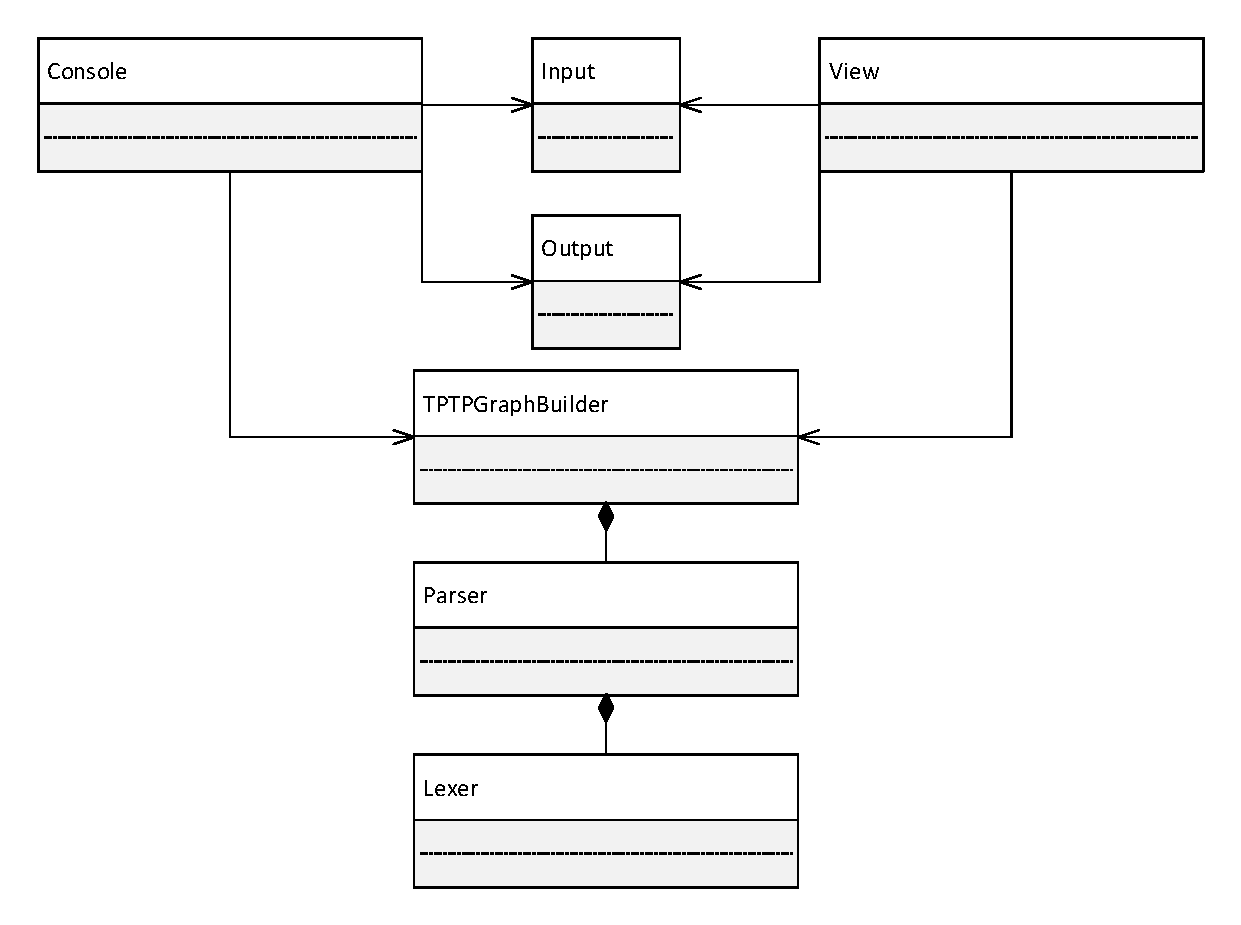
\includegraphics[width=1\textwidth]{images/Concept_UML_Architecture_Overview.pdf}
\caption{UML diagram of the architecture of the software tool}
\label{fig:ConceptArchitectureOverview}
\end{figure}
\subsection{Implementation language}\label{sec:ConceptImplementationLanguage}
todo why python

\section{Lexer}\label{sec:ConceptLexer}
The lexer is responsible for extracting tokens from the TPTP language grammar specification file. Using \ac{PLY} a lexer can be built by specifying tokens as regular expressions.\\
Therefore the TPTP language grammar specification needs to be analysed in order to find elementary tokens and regular expressions, that precisely describe these
tokens. 

%\subsubsection{Token identification}\label{sec:ConceptElementaryTokens}
%The syntax of the \ac{TPTP} language is specified in a modified \ac{EBNF} \ref{VS06}.
%Therefore there are deviations from standard \ac{EBNF} (see \ref{sec:BackgroundBNF}) that need to be analysed to specify elementary tokens.
%The standard \ac{EBNF} only uses one production symbol ($"::="$).
%In the \ac{TPTP} syntax additional production symbols have been added.
%The following table \ref{tbl:ConceptTPTPProductionSymbols} contains the production symbols used in the \ac{TPTP} syntax, that also have to be recognized by the lexer.
%\begin{table}[H]
%\centering
%\renewcommand{\arraystretch}{1}
%\caption{\ac{TPTP} language production symbols \cite{VS06}}
%\begin{tabular}{ll}
%\textbf{Symbol} & \textbf{Rule Type}\\\hline
%::= & Grammar\\
%:== & Strict\\
%::- & Token\\
%::: & Macro\\
%\end{tabular}
%\label{tbl:ConceptTPTPProductionSymbols}
%\end{table}
%
%Another deviation from \ac{EBNF} is that repetition is not denoted by surrounding curly brackets, but with a trailing $*$ symbol.\\
%Curly brackets have no special meaning in the \ac{TPTP} syntax and can be treated as terminal symbols.\\
%The meaning of the alternative symbol $|$ is unchanged and also parentheses and square brackets can appear as meta symbols.\\
%Also, there are line comments in the \ac{TPTP} syntax.
%A comment starts with the $\%$ symbol at the beginning of a line and ends at the end of that line.\\
%Following standard \ac {BNF}, nonterminal symbols are enclosed by the $<$ and $>$ symbol and terminal symbols are written without any special marking.

The standard extended BNF only uses one production symbol ($"::="$).
In the TPTP syntax the standard production symbol is used for syntactic rules.
Additional symbols for semantic, lexical and character-macro rules have been added.
The following table contains the production symbols for grammar (syntactic rules), strict (semantic rules), token (lexical rules) and macro (character-macro rules) rule types used in the TPTP syntax.

\begin{table}[H]
\centering
\renewcommand{\arraystretch}{1}
\caption{\ac{TPTP} language rule types \cite{VS06}}
\begin{tabular}{ll}
\textbf{Symbol} & \textbf{Rule Type}\\\hline
::= & Grammar\\
:== & Strict\\
::- & Token\\
::: & Macro\\
\end{tabular}
\label{tbl:ConceptTPTPProductionSymbols}
\end{table}


%The identified token types will be explained in the following.
The following paragraph introduces the tokens that are recognized by the lexer. Tokens are written bold.

Following standard BNF, \textbf{nonterminal} symbols are enclosed by the \textless\; and \textgreater \;symbol.
In between there can be any arbitrary sequence of alphanumerical characters and underscores.

A \textbf{terminal symbol} does not have any special notation and ?is matched if none of the other tokens are matched?.
%Every sequence of characters that does not start with \textless\; and does not end with \textgreater is a \textit{terminal symbol}.

There are four \textbf{expression} token types (one for each rule type).
\textbf{Expressions} are defined as a nonterminal symbol followed by a production symbol (::= for grammar, ::- for token, :== for strict, ::: for macro rule type).
The nonterminal symbol and the following production symbol are selected to be a single token and are not identified as two separate tokens to clearly identify the start of a new rule and therefore avoid ambiguity while parsing.
The example below features two tokens, a grammar expression and a nonterminal symbol.
\begin{verbatim}
<formula_role>         ::= <lower_word>
\end{verbatim}

A \textbf{comment} is defined as the start of a new line, a percentage sign, arbitrary characters and ends with a newline character.
The percentage sign when used as terminal symbol is embedded in square brackets and can therefore never be the first character of a new line.

Additional tokens are the meta-symbols including \textbf{open} $"("$ and \textbf{close parentheses} $")"$, \textbf{open} $"["$ and \textbf{close square brackets} $"]"$, asterisks $"*"$ called \textbf{repetition symbols} and vertical bars $"\mid"$ called \textbf{alternative symbols}.

In PLY it is possible to declare characters that should be ignored. This means that the characters would be ignored in the input stream of the lexer. However, if one of those characters are part of a regular expression they are not ignored and will be used for token matching. In this project tabs, white spaces and newline characters are ignored as they do not have any special meaning other than providing better readability. With exception of the comment token, the information about newline characters is not relevant due to rules being defined over multiple lines, which can be seen in the example below.
\begin{verbatim}
<annotated_formula>  ::=    <thf_annotated> | <tff_annotated> |
                            <tcf_annotated> | <fof_annotated> |
                            <cnf_annotated> | <tpi_annotated>
\end{verbatim}


\section{Parser}\label{sec:ConceptParser}
The parser takes the tokens from the lexer as input and creates a data structure that represents the structure of the \ac{TPTP} syntax.

Figure \ref{fig:ConceptParserFlow} outlines the responsibilities of the parser component and the sequence of its sub-functions.
First, the tokens generated by the lexer need to be parsed and based on that the data structure representing the \ac{TPTP} syntax is to be created.
The rules in the data structure have to be numbered, to maintain the correct order for output, after creating the grammar tree in the next step (see section \ref{sec:Concept}).

In the \ac{TPTP} syntax square brackets not necessarily denote that an expression is optional, which is the case in traditional \ac{EBNF} .
In token and macro rules they denote that an expression is optional and in grammar and strict rules square brackets are terminals.
Therefore disambiguation of square brackets is necessary.
\begin{figure}[H]
\tikzstyle{decision} = [ diamond, draw, fill=blue!10, text width=4.5em, text badly centered, node distance=2cm, inner sep-0pt]  
\tikzstyle{block} = [ rectangle, draw, fill=blue!10, text width=5em, text badly centered, rounded corners, minimum height=4em]  
\tikzstyle{line} = [ draw, -latex']  
%\tikzstyle{terminator} = [ draw, ellipse, fill=red!20, node distance=3cm, minimum height=2em]
\tikzstyle{terminator} = [rectangle, draw, fill=blue!10, text width=5em, text badly centered, rounded corners, minimum height=4em]  
\begin{center}
\begin{tikzpicture}[node distance=3cm, auto]  
  \node [terminator]  (start)  {Parse tokens};  
  \node [block, right of=start]  (number) {Number rules};  
  \node [block, right of=number] (disambigue) {Disambigue square brackets}; 
  \node [block, right of=disambigue] (return) {Return result}; 
 
  \path [line] (start)  -- (number);  
  \path [line] (number) -- (disambigue);  
  \path [line] (disambigue) -- (return); 
\end{tikzpicture}
\end{center}
\caption{Parsing procedure}
\label{fig:ConceptParserFlow}
\end{figure}

\subsection{Data structures and data types}\label{sec:ConceptParserDataStructure}
To build the representative data structure, data types that represent the data stored in the \ac{TPTP} syntax have to be defined.
The following section describes the data structure and data types that are used and created by the parser in the parsing process.

%Atomic data types

\subsubsection{Terminal symbol}
The terminal symbol data type has one attribute, which is the name of the terminal symbol it represents.

-todo Production Property

\subsubsection{Nonterminal symbol}
Analogue to the terminal symbol data type, the nonterminal symbol also has its name as an attribute.

todo describe diagram
\begin{figure}[H]
\centering
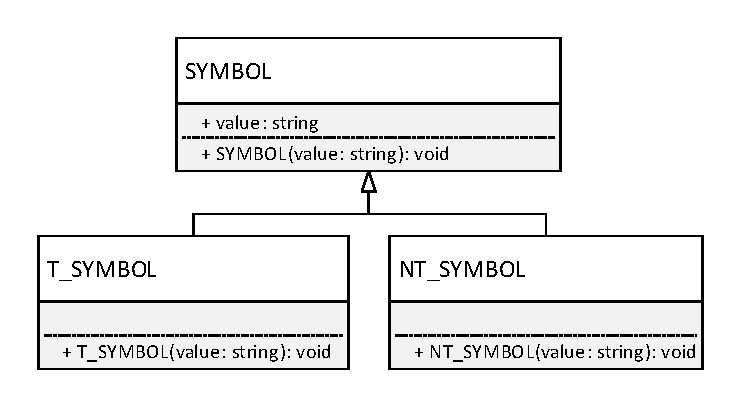
\includegraphics[width=.8\textwidth]{images/Concept_uml_data_types_symbols.pdf}
\caption{Symbol data type UML class diagram}
\label{fig:ConceptSymbolsClassDiagram}
\end{figure}
%Composite data types

\subsubsection{Rules}
%\subsubsection{Grammar Expression}
A rule consists of the nonterminal symbol name which is produced, a production list and a position.
The position denotes at which position in the \ac{TPTP} syntax the rule was listed.
This information is needed to maintain the original order of the rules when printing the reduced syntax.\\
For each rule type (see table \ref{tbl:ConceptTPTPProductionSymbols}) there is a data type.
This means that grammar, token, strict and macro rule data types are introduced.\\
Listing \ref{lst:ConceptParserGrammarExpression} contains an example of a line in a \ac{TPTP} syntax file that is represented by the grammar rule data type.
The nonterminal symbol name which is produced is <$tff \textunderscore formula$>.  The production list consists of two productions, as can be seen in the listing.
\begin{lstlisting}[basicstyle=\scriptsize	,caption= Grammar expression,label= lst:ConceptParserGrammarExpression]
<tff_formula>          ::= <tff_logic_formula> | <tff_atom_typing
\end{lstlisting}


todo describe diagram
\begin{figure}[H]
\centering
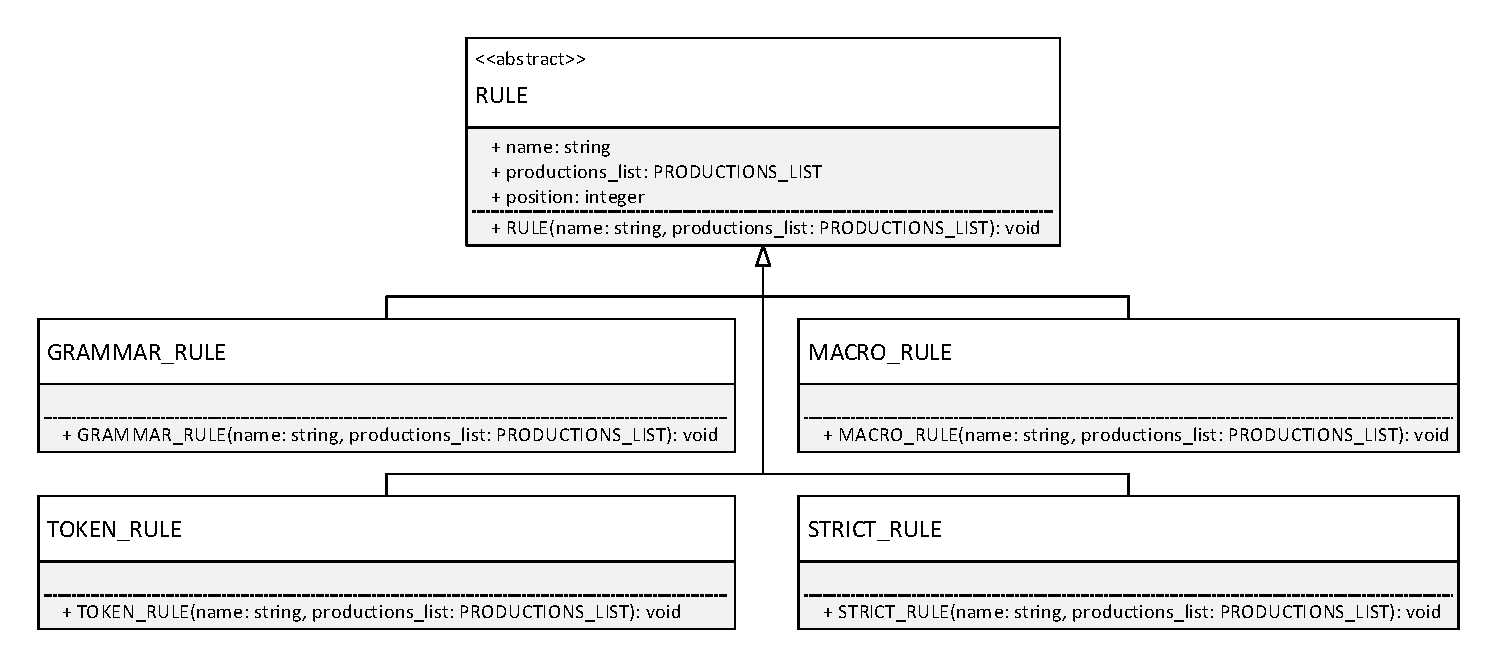
\includegraphics[width=1\textwidth]{images/Concept_uml_data_types_rules.pdf}
\caption{Rule data type UML class diagram}
\label{fig:ConceptRulesClassDiagram}
\end{figure}

\subsubsection{Comment block}
A comment block is a list of consecutive comment lines.

todo describe diagram
\begin{figure}[H]
\centering
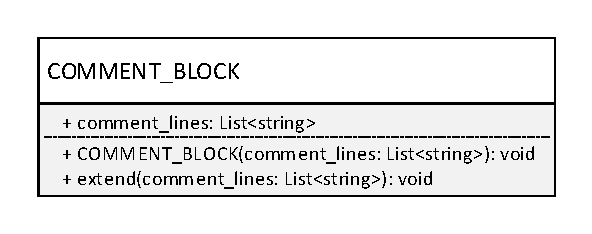
\includegraphics[width=.5\textwidth]{images/Concept_uml_data_types_comment_block.pdf}
\caption{Comment block data type UML class diagram}
\label{fig:ConceptCommentBlockClassDiagram}
\end{figure}

\subsubsection{Production element}
A production element is either a terminal or nonterminal symbol. Additionally a production symbol has a production property.
\begin{figure}[H]
\centering
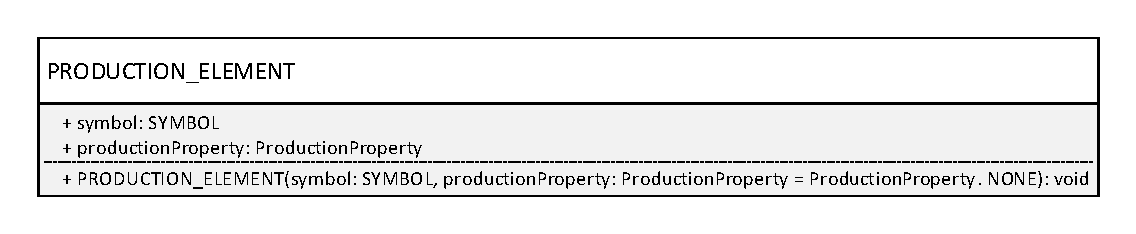
\includegraphics[width=.8\textwidth]{images/Concept_uml_data_types_production_element.pdf}
\caption{Production element data type UML class diagram}
\label{fig:ConceptProductionElementClassDiagram}
\end{figure}

\subsubsection{Production property}
The production property can take one of three values and denotes whether a production is optional, can be repeated any number of times or does not have any special property.
In the original \ac{TPTP} syntax file this was represented by square brackets or the repetition symbol.

todo describe diagram
\begin{figure}[H]
\centering
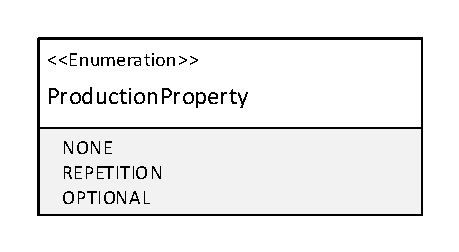
\includegraphics[width=.4\textwidth]{images/Concept_uml_data_types_production_property.pdf}
\caption{Production property data type UML class diagram}
\label{fig:ConceptProductionPropertyClassDiagram}
\end{figure}

\subsubsection{Production}
A production is one production alternative specified in any expression.
It consists of a list of production elements and has a production property. Productions can also be nested.
Therefore the list can also contain further productions

-show example
\begin{figure}[H]
\centering
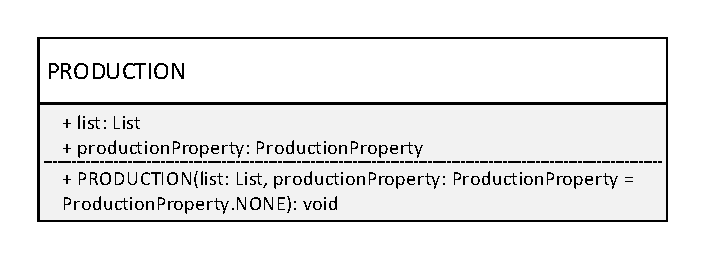
\includegraphics[width=.5\textwidth]{images/Concept_uml_data_types_production.pdf}
\caption{Production data type UML class diagram}
\label{fig:ConceptProductionClassDiagram}
\end{figure}

\subsubsection{Productions list}
A productions list contains a list of productions where each production is one alternative in the description of an expression.


\subsubsection{XOR Productions list}
The XOR productions list represents multiple alternatives enclosed by parentheses. It contains a list of the alternate productions.
 
 todo describe diagram
\begin{figure}[H]
\centering
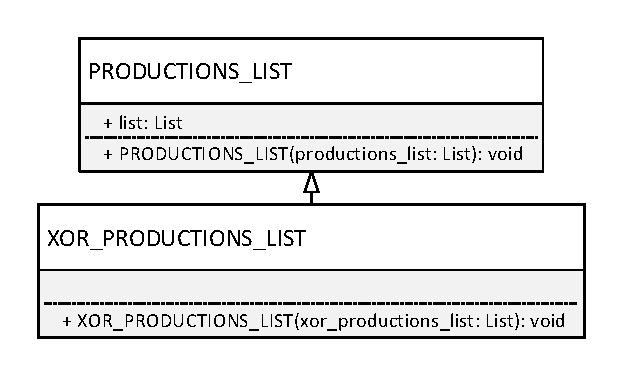
\includegraphics[width=.6\textwidth]{images/Concept_uml_data_types_productions_list.pdf}
\caption{Productions list data type UML class diagram}
\label{fig:ConceptProductionsListClassDiagram}
\end{figure}

\subsubsection{Grammar list}
The grammar list is the top level data structure. It contains a list of all elements that were in the \ac{TPTP} syntax file.
This includes any type of rules (grammar, token, strict and macro) and comment blocks.

todo describe diagram
\begin{figure}[H]
\centering
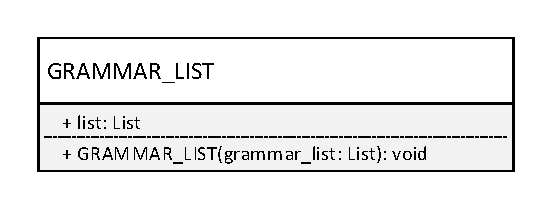
\includegraphics[width=.5\textwidth]{images/Concept_uml_data_types_grammar_list.pdf}
\caption{Grammar list data type UML class diagram}
\label{fig:ConceptGrammarListClassDiagram}
\end{figure}
\subsection{Production rules}
When using the \ac{PLY} parser generator, production rules have to be defined.
The rules describe how the tokens are to be processed.

todo describe production rules

\subsection{Disambiguation of  square brackets}
As mentioned before, square brackets have different meanings depending on the rule type.
The idea to solve this problem is to treat all rules the same in the first processing step.
Square brackets would then be interpreted as denoting the optional production property.
This production property would then be selected for productions that are enclosed by square brackets for all types of rules.
In an additional processing step, after creating the grammar list each grammar and strict rule can be iterated, exchanging the production property optional by the square bracket terminal symbols.

todo vor- nachteile


The output of the parser is a list of the rules and the comments from the \ac{TPTP} syntax file.
\section{Graph generation}\label{sec:ConceptGraphGeneration}
After parsing the TPTP grammar is stored in a grammar list. The grammar list data structure does not allow traversing which is why a new data structure is introduced that allows for modification and traversing.
The data structure that is used is a graph representing the grammar.

The nonterminal symbols in the TPTP syntax are represented by a node class that has the following attributes:
\begin{itemize}
\item value: name of nonterminal symbol
\item productions list: productions list of nonterminal symbol (todo created by the parser)
\item rule type: rule type of nonterminal symbol
\item comment block: list of comments belonging to the nonterminal symbol
\item position: position of the production in the input file
\item children: nested list, containing lists of all nonterminating symbols per production
\end{itemize}

Before generating the graph, a dictionary is created.
This dictionary contains nodes constructed from the grammar list output by the parser that contains rules and comments.
While constructing the dictionary, comments in the grammar list are associated to nodes using a heuristic that is described in section \ref{sec:ConceptMaintainingComments}.
The combination of the nodes' value and rule type form the unique key for each node.
The dictionary provides an efficient way accessing them in order to build the grammar graph and also during the next step of sub-syntax generation.

Also, a new temporary start symbol is introduced.
This is necessary because one nonterminal symbol in the TPTP syntax can be mapped to multiple nodes.
The example below shows the productions for the nonterminal symbol $\textless formula\textunderscore role\textgreater$.
Since this nonterminal symbol has multiple types of rules one node will be created for each rule type.

\begin{verbatim}
<formula_role>         ::= <lower_word>
<formula_role>         :== axiom | hypothesis | definition | assumption |
                           lemma | theorem | corollary | conjecture |
                           negated_conjecture | plain | type |
                           fi_domain | fi_functors | fi_predicates | unknown
\end{verbatim}

If a nonterminal symbol that has multiple rule types is selected as the desired start symbol multiple nodes would represent that start symbol and therefore it would not be possible to select one node as the starting point of the graph generation.
To solve this problem, the temporary start symbol is introduced before graph generation.
This start symbol produces the start symbol that the user specified and is used as a starting point for the graph generation.
If the before mentioned nonterminal symbol $\textless formula\textunderscore role\textgreater$ would be selected as start symbol by the user a temporary start symbol representing the rule
\begin{verbatim}
<start_symbol>         ::= <formula_role>
\end{verbatim}
would be introduced.
This ensures that only one node is representing the start symbol, that is used for graph generation.

Starting with the temporary start symbol, the graph is generated recursively. Iterating over each nonterminal symbol in the productions list of the start symbol, the corresponding nodes are identified. These nodes are then appended to the list of children of the start symbol. The identified children may again have children. This process is repeated until a node has no children because there are only terminal symbols in the productions list of a nonterminal symbol.

Since it is possible for a nonterminal symbol to be on the right side as well as on the left side of the same production rule, a node can also be its own child. To avoid revisiting the same node infinitely, it is checked whether a node already has children so that it will not be visited again. This also improves the performance of the tool as a nonterminal symbol that has already been visited wont be visited again independent of circular dependencies.

The following example shows a production rule and the resulting list of children belonging to the node. Each production alternative has its own list of children. %This is relevant for checking whether a nonterminal is terminating.
\begin{verbatim}
Production rule:
<disjunction>  ::=  <literal> | <disjunction><vline><literal>
Output:
node.value: <disjunction>
node.ruleType: grammar
node.children: [[<literal>],[<disjunction>,<vline>,<literal>]]
\end{verbatim}

\section{Control file}\label{sec:ConceptControlFile}
In the following section a format for specifying the desired start symbol and blocked productions is described.
Using a file-based configuration enables the user to store desired configurations and for example a manual selection in the graphical user interface is not necessary.
It also helps with using the command line interface, because there manual selection is not possible.
The file should be human-readable and -editable.\\
The format should be easy to parse and allow to specify all necessary information.
This includes the desired start symbol and all production rules that should be blocked.\\
The proposed way to describe this information is to:

\begin{itemize}%[noitemsep]
	\item define the desired start symbol in the first line.
	\item define blocked productions grouped by nonterminal symbol and production symbol separating each group by a new line.
	First defining the nonterminal symbol, then the production symbol and after that the index of the alternatives that should be blocked (indexing starts at zero). 
\end{itemize}

Identifying the production symbol is necessary because there may be a nonterminal symbol that has productions with more than one production symbol.\\
Listing \ref{lst:ConceptControlFile} contains a sample control file. In this file in the first line <$TPTP\_file$> is specified as start symbol.
The second line means, that the second grammar production alternative of the nonterminal symbol <$TPTP\_input$> should be disabled.
Analogue to that, the first, second, third and fifth grammar production alternative of the nonterminal symbol <$annotated\_formula$> are said to be disabled in line 3.

\begin{lstlisting}[caption= Control file,label= lst:ConceptControlFile]
<TPTP_file>
<TPTP_input>,::=,1
<annotated_formula>,::=,0,1,2,5
\end{lstlisting}
This format is relatively easy to parse and also enables users to specify their desired start symbols and blocked productions without having to use the GUI.

pro: Specifying which production should be blocked, and not the ones should be kept, typically results in a significantly smaller file.
Storing the indexes of the productions that should be blocked offers that in case productions are renamed the control file would still be valid. On the other hand if productions are added or deleted from the original \ac{TPTP} syntax, the control file may have to be updated.

\section{Maintaining comments}\label{sec:ConceptMaintainingComments}
In the \ac{TPTP} syntax there are comments providing supplemental information about the language and its symbols and rules.
When generating a reduced grammar maintaining comments is desired. This means that comments from the original language specification should be associated with the rule they belong to and if the rule is still present in the reduced grammar, also the comment should be.\\
Therefore a mechanism has to be designed for the association of comments to grammar rules.

Listing \ref{lst:ConceptComment_tptp} features an example of a comment in a \ac{TPTP} syntax file. This comment begins with a \textit{Top of Page} line which, in the HTML version of the \ac{TPTP} syntax, contains a hyperlink which leads to the beginning of the syntax file.
The next line contains a relevant comment.\\
\begin{lstlisting}[language=none, basicstyle=\scriptsize	,caption= Comment in the \ac{TPTP} syntax,label= lst:ConceptComment_tptp]
%----Top of Page---------------------------------------------------------------
%----TFF formulae.
<tff_formula>          ::= <tff_logic_formula> | <tff_atom_typing> |
                           <tff_subtype> | <tfx_sequent>
\end{lstlisting}
todo check if listing is handled correctly

The heuristic matching comments to rules takes these \textit{Top of Page} lines into account.
When there is a \textit{Top of Page} line in between comment lines it generally also splits comments sematically. todo maybe proof
In listing \ref{lst:ConceptComment_tptp} can be seen that the comment in line 2 refers to the rule after.
Therefore it would be correct to associate the comment line after the \textit{Top of Page} line to the rule after.
Also, if there is one \textit{Top of Page} line in between multiple comment lines it is highly probable that the first part of the comment lines before the \textit{Top of Page} line refer to the rule before the comments and that the lines after the \textit{Top of Page} line refer to the rule after the comment lines.
This scenario can be seen in listing \ref{lst:Comment_split_example}.
The \textit{Top of Page} line is in line 28 and the comment lines before refer to the rule before.
The comment line after refers to the rule after that line.
\begin{lstlisting}[language=none, basicstyle=\scriptsize	,caption=Comment lines split by a \textit{Top of Page} line in the \ac{TPTP} syntax,label= lst:Comment_split_example]
<formula_role>         :== axiom | hypothesis | definition | assumption |
                           lemma | theorem | corollary | conjecture |
                           negated_conjecture | plain | type |
                           fi_domain | fi_functors | fi_predicates | unknown
%----"axiom"s are accepted, without proof. There is no guarantee that the
%----axioms of a problem are consistent.
%----"hypothesis"s are assumed to be true for a particular problem, and are
%----used like "axiom"s.
%----"definition"s are intended to define symbols. They are either universally
%----quantified equations, or universally quantified equivalences with an
%----atomic lefthand side. They can be treated like "axiom"s.
%----"assumption"s can be used like axioms, but must be discharged before a
%----derivation is complete.
%----"lemma"s and "theorem"s have been proven from the "axiom"s. They can be
%----used like "axiom"s in problems, and a problem containing a non-redundant
%----"lemma" or theorem" is ill-formed. They can also appear in derivations.
%----"theorem"s are more important than "lemma"s from the user perspective.
%----"conjecture"s are to be proven from the "axiom"(-like) formulae. A problem
%----is solved only when all "conjecture"s are proven.
%----"negated_conjecture"s are formed from negation of a "conjecture" (usually
%----in a FOF to CNF conversion).
%----"plain"s have no specified user semantics.
%----"fi_domain", "fi_functors", and "fi_predicates" are used to record the
%----domain, interpretation of functors, and interpretation of predicates, for
%----a finite interpretation.
%----"type" defines the type globally for one symbol; treat as $true.
%----"unknown"s have unknown role, and this is an error situation.
%----Top of Page---------------------------------------------------------------
%----THF formulae.
<thf_formula>          ::= <thf_logic_formula> | <thf_atom_typing> |
                           <thf_subtype> | <thf_sequent>
\end{lstlisting}

The flow chart in figure \ref{fig:ConceptMaintainingComments} shows the process of matching comment blocks, that are consecutive comment lines (see section \ref{sec:ConceptParserDataStructure}),  to rules.
First, the comment block is split into multiple separate comment blocks by using \textit{Top of Page} lines as separators.
\begin{itemize}%[noitemsep]
	\item If this results in no comment blocks the comment block consisted only of one line which was a \textit{Top of Page} line.
	Then no comment block has to be associated to a rule because \textit{Top of Page} lines are not relevant.
	\item If this results in one comment block, that means that no \textit{Top of Page} line was present in the comment block and the comment block is associated with the rule after, if the comment block is not at the end of the file.
	If it is at the end of the file it is associated with the rule before. todo why
	\item If this results in two comment blocks, one \textit{Top of Page} line was present.
	Then the comment block before the \textit{Top of Page} line is associated with the rule before when possible.
	If this comment block is at the beginning of the file it is associated with the rule after.
	The comment block after the \textit{Top of Page} line is associated with the rule after.
	If it is at the end of the file it is associated with the rule before.
\end{itemize}
The case of three or more comment blocks after splitting the original comment block is not featured in the flow chart.
This case does not occur in the \ac{TPTP} syntax version 7.3.0.
Therefore it is not particularly relevant.
Since it might occur in a future version of the \ac{TPTP} syntax it is handled by merging all comment blocks starting from the second and then following the procedure of two comment blocks in the flow chart in figure \ref{fig:ConceptMaintainingComments}.

\begin{figure}[H]
\centering
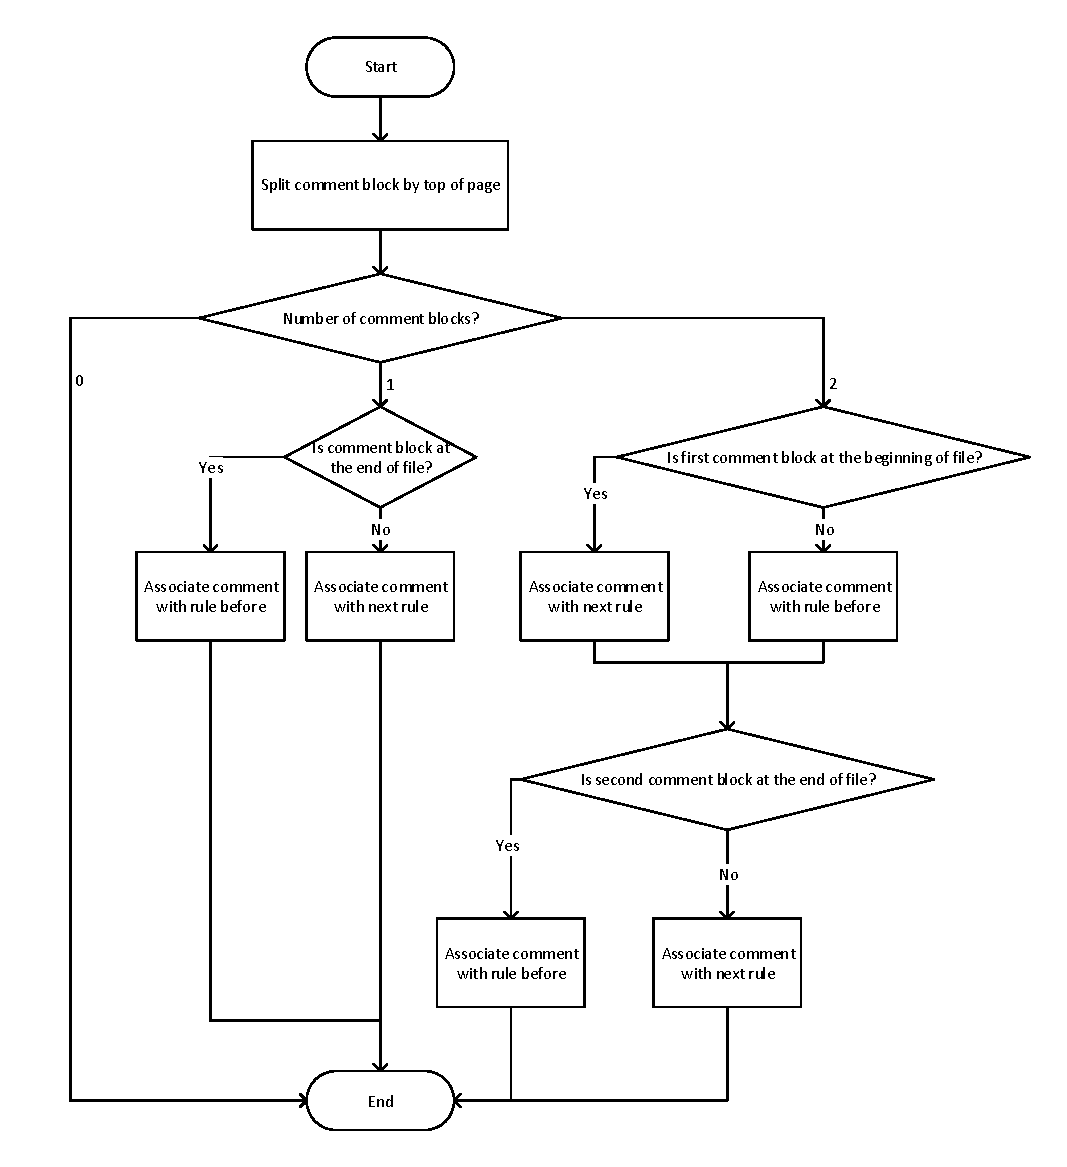
\includegraphics[width=1\textwidth]{images/Concept_maintaining_comments.pdf}
\caption{Maintaining comments flow chart}
\label{fig:ConceptMaintainingComments}
\end{figure}
todo describe split comment block by top of page

todo explain could use content of comment

\section{Extraction of a sub-syntax}\label{sec:ConceptExtractReducedGrammar}
This section covers the concept of how a sub-syntax is computed from the original syntax.
The original syntax is represented by a grammar graph (see section \ref{sec:ConceptGraphGeneration}) and the information on what part of the syntax to extract is described in a control file.
To extract a sub-syntax from the original grammar graph, four steps must be performed:
\begin{enumerate}%[noitemsep]
	\item The control file has to be parsed, in order to get information on the desired start symbol and which productions should be blocked
	\item The blocked productions specified in the control file must be disabled and therefore the corresponding transitions must be removed from the grammar graph.
	\item The remaining reachable part of the grammar must be computed.
	\item Starting from the still reachable part of the grammar, non terminating productions must be removed.
\end{enumerate}
\subsection{Parsing a control file}\label{sec:ConceptParsingControlFile}
The control file provides the necessary information for the extraction of a sub-syntax.
The format of the control file is described in section \ref{sec:ConceptControlFile}. 
The start symbol is listed in the first line.
Every consecutive line contains a nonterminal symbol, the corresponding rule type symbol, and the indexes of the productions that should be blocked separated by comma.
The start symbol will be relevant in determining the remaining reachable part of the grammar (section \ref{sec:ConceptDerterminingRemainingReachable}) whereas the information on the productions that should be blocked will be needed in the next section.

\subsection{Removal of blocked productions}\label{sec:ConceptRemovingBlockedProductions}
In the control file, for each nonterminal symbol, whose productions should be modified, its name, rule type and the indexes of the productions that should be blocked are listed.
From all nodes, that are adressed (by nonterminal symbol name and rule type), the indexed productions are removed.
This includes deleting the corresponding element from the productions list and from the children list.

\subsection{Determination of the remaining terminating symbols}\label{sec:ConceptDerterminingRemainingTerminating}
After all reachable symbols have been determined, the last step of extracting a sub-syntax is to determine and remove the non-terminating productions and symbols.
Non-terminating productions are productions in which at least one nonterminal symbol is non-terminating.\\

The terminating symbols can be determined recursively using dynamic programming techniques.
The goal is to determine for each nonterminal symbol if it derives a terminating symbol. Only then it is a useful symbol since it is reachable and derives a terminating symbol todo reference
Starting at the start symbol, the grammar graph is traversed. 

-start with start symbol
-traverse through graph and compute terminating symbols
- store visited nodes to avoid infinite loops

\subsection{Determination of the remaining reachable symbols}\label{sec:ConceptDerterminingRemainingReachable}
After removing the productions specified in the control file it has to be determined which part of the grammar still remains reachable.
This is done by generating a new grammar graph starting from desired the start symbol.
When generating the new grammar graph, all from the start symbol reachable parts of the grammar will be added to the new grammar graph (see section \ref{sec:ConceptGraphGeneration}).
All nodes that are not part of the new grammar graph are not reachable and can therefore be removed.

\section{Output generation}\label{sec:ConceptOutputGeneration}
Internally in the software tool a syntax is represented by a grammar graph.
To make sub-syntaxes represented by a grammar graph usable they have to be converted to the original form of a \ac{TPTP} syntax file. This process is described in the following subsection.
After that measures to provide compatibility with the automated parser generator are discussed in section \ref{sec:ConceptAutomatedParserGenerator}.

\subsection{Create output from grammar graph}\label{sec:ConceptOutputGrammarGraph}
There are three steps necessary in order for 
\begin{figure}[H]
\tikzstyle{decision} = [ diamond, draw, fill=blue!10, text width=4.5em, text badly centered, node distance=2cm, inner sep-0pt]  
\tikzstyle{block} = [ rectangle, draw, fill=blue!10, text width=10em, text badly centered, rounded corners, minimum height=4em]  
\tikzstyle{line} = [ draw, -latex']  
\tikzstyle{terminator} = [rectangle, draw, fill=blue!10, text width=10em, text badly centered, rounded corners, minimum height=4em]  
\begin{center}
\begin{tikzpicture}[node distance=5.5cm, auto]  
  \node [terminator]  (traverse)  {Traverse grammar graph and get nodes strings and positions};  
  \node [block, right of=traverse]  (order) {Order nodes strings by positions};  
  \node [terminator, right of=order] (store) {Store ordered nodes strings in file}; 

  \path [line] (traverse)  -- (order);  
  \path [line] (order) -- (store);  
\end{tikzpicture}
\end{center}
\caption{Procedure of generating a Syntax string representation from the grammar graph}
\label{fig:ConceptOutputGrammarGraphProcedure}
\end{figure}
- iterate over nodes and get string representation of nodes with node position
- store node string with position
- order node strings by position


- print to file
-recursive

- each node represents rule of certain rule type with possibly multiple production alternatives

-recursively build strings

-maintain order of rules

-temporary start symbol pos -1 to not print

\subsection{Automated parser generator compatibility}\label{sec:ConceptAutomatedParserGenerator}
The automated parser generator for the \ac{TPTP} syntax \cite{VS06} takes a \ac{TPTP} syntax file as input and creates a lex and yacc file corresponding to the specification in the input syntax.\\
In the \ac{TPTP} syntax version 7.3.0 there is a definition of the syntax of comments which is shown in listing \ref{lst:ConceptAutomatedParserGeneratorComment}.
\begin{lstlisting}[language=none, basicstyle=\scriptsize, caption=Comment syntax definition in the \ac{TPTP} syntax, label= lst:ConceptAutomatedParserGeneratorComment]
<comment>              ::- <comment_line>|<comment_block> 
<comment_line>         ::- [%]<printable_char>*
<comment_block>        ::: [/][*]<not_star_slash>[*][*]*[/]
<not_star_slash>       ::: ([^*]*[*][*]*[^/*])*[^*]*
<printable_char>       ::: .
\end{lstlisting}

However this part of the syntax is not reachable from any other symbol.
When constructing the grammar graph this part of the syntax is therefore removed.\\
Using a syntax file, in which the comment syntax is not present, with the automated parser generator results in an error because the comment symbol is not present in the lex specification but is referred to in a yacc rule ?todo check this?.\\
There are two ways to include the comment syntax in the output from the tool in order to be accepted by the automated parser generator.
Either making the \textit{<comment>} nonterminal symbol reachable by for example by adding it as an alternative to \textit{<TPTP\textunderscore input>} which can be seen in listing \ref{lst:ConceptAutomatedParserGeneratorCommentReachable}.
Or maintaining the comment syntax separately and adding it to the output syntax even though it is not reachable.
\begin{lstlisting}[language=none, basicstyle=\scriptsize, caption=Making the comment syntax reachable, label= lst:ConceptAutomatedParserGeneratorCommentReachable]
<TPTP_file>            ::= <TPTP_input>*
<TPTP_input>           ::= <annotated_formula> | <include> | <comment>
\end{lstlisting}

Both ways are supported by the tool.\\
If the \textit{<comment>} nonterminal symbol is made reachable in the \ac{TPTP} syntax, the grammar graph generated by the tool contains the comment syntax and no further action is necessary.\\
To add the comment syntax to the output if the is \textit{<comment>} nonterminal symbol is not reachable is done by using an external configuration file that contains the syntax from listing \ref{lst:ConceptAutomatedParserGeneratorComment}.
From the syntax in this configuration file a separate grammar graph is generated. The output string that can be generated from this grammar graph is added to the output of the tool when outputting a generated sub-syntax.

-Menu option

-comment symbol in lex

-make comment reachableto be tested
\section{GUI}\label{sec:ConceptGUI}
The graphical user interface is built using PyQt. Advantages of PyQT are that it offers a treeview that is used for displaying the grammar. In comparison to the standard Python library Tkinter PyQt offers checkboxes in treeviews \cite{Tkinter} that are used for selecting blocked productions.

todo
In this section ...
 
-Tkinter and PyQt have been evaluated
-Tikinter does not offer a kind of table view with checkboxes
-which PyQt offers natively
The graphical user interface should display the grammar similar to the original language grammar specification file.
It should also be possible to make selections in the GUI instead of having to use a control file. 
-show rules similar to file
Selection of a new start symbol and productions that should be possible in the GUI and also with the import of a control file.

The menu of the GUI consists of four submenus.

The $Import$ menu that can be seen in figure \ref{fig:import} provides the option to import a TPTP syntax file in txt file format from local storage or to import the latest TPTP syntax version from the TPTP website.
The TPTP syntax on the TPTP project website is stored in a HTML format.
This file is downloaded and converted to plain text using the Beautiful Soup Python library \cite{BeautifulSoup}.

\begin{figure}[H]
\centering
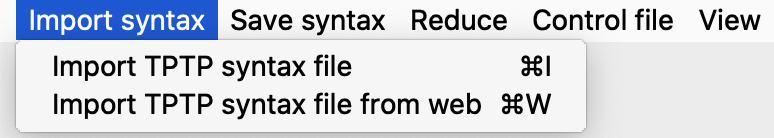
\includegraphics[width=.7\textwidth]{images/import.png}
\caption{Import menu}
\label{fig:import}
\end{figure}

After selecting a file for import a start symbol needs to be selected.
Starting with the start symbol a grammar graph is generated and the corresponding text displayed.
Each rule in the TPTP grammar is a top element of the treeview and can be expanded to show the productions alternatives.
Right of the nonterminals name the rule type is displayed.
Comments that have been assigned to a rule are also displayed. An example of the imported TPTP grammar is shown in figure \ref{fig:gui}.

\begin{figure}[H]
\centering
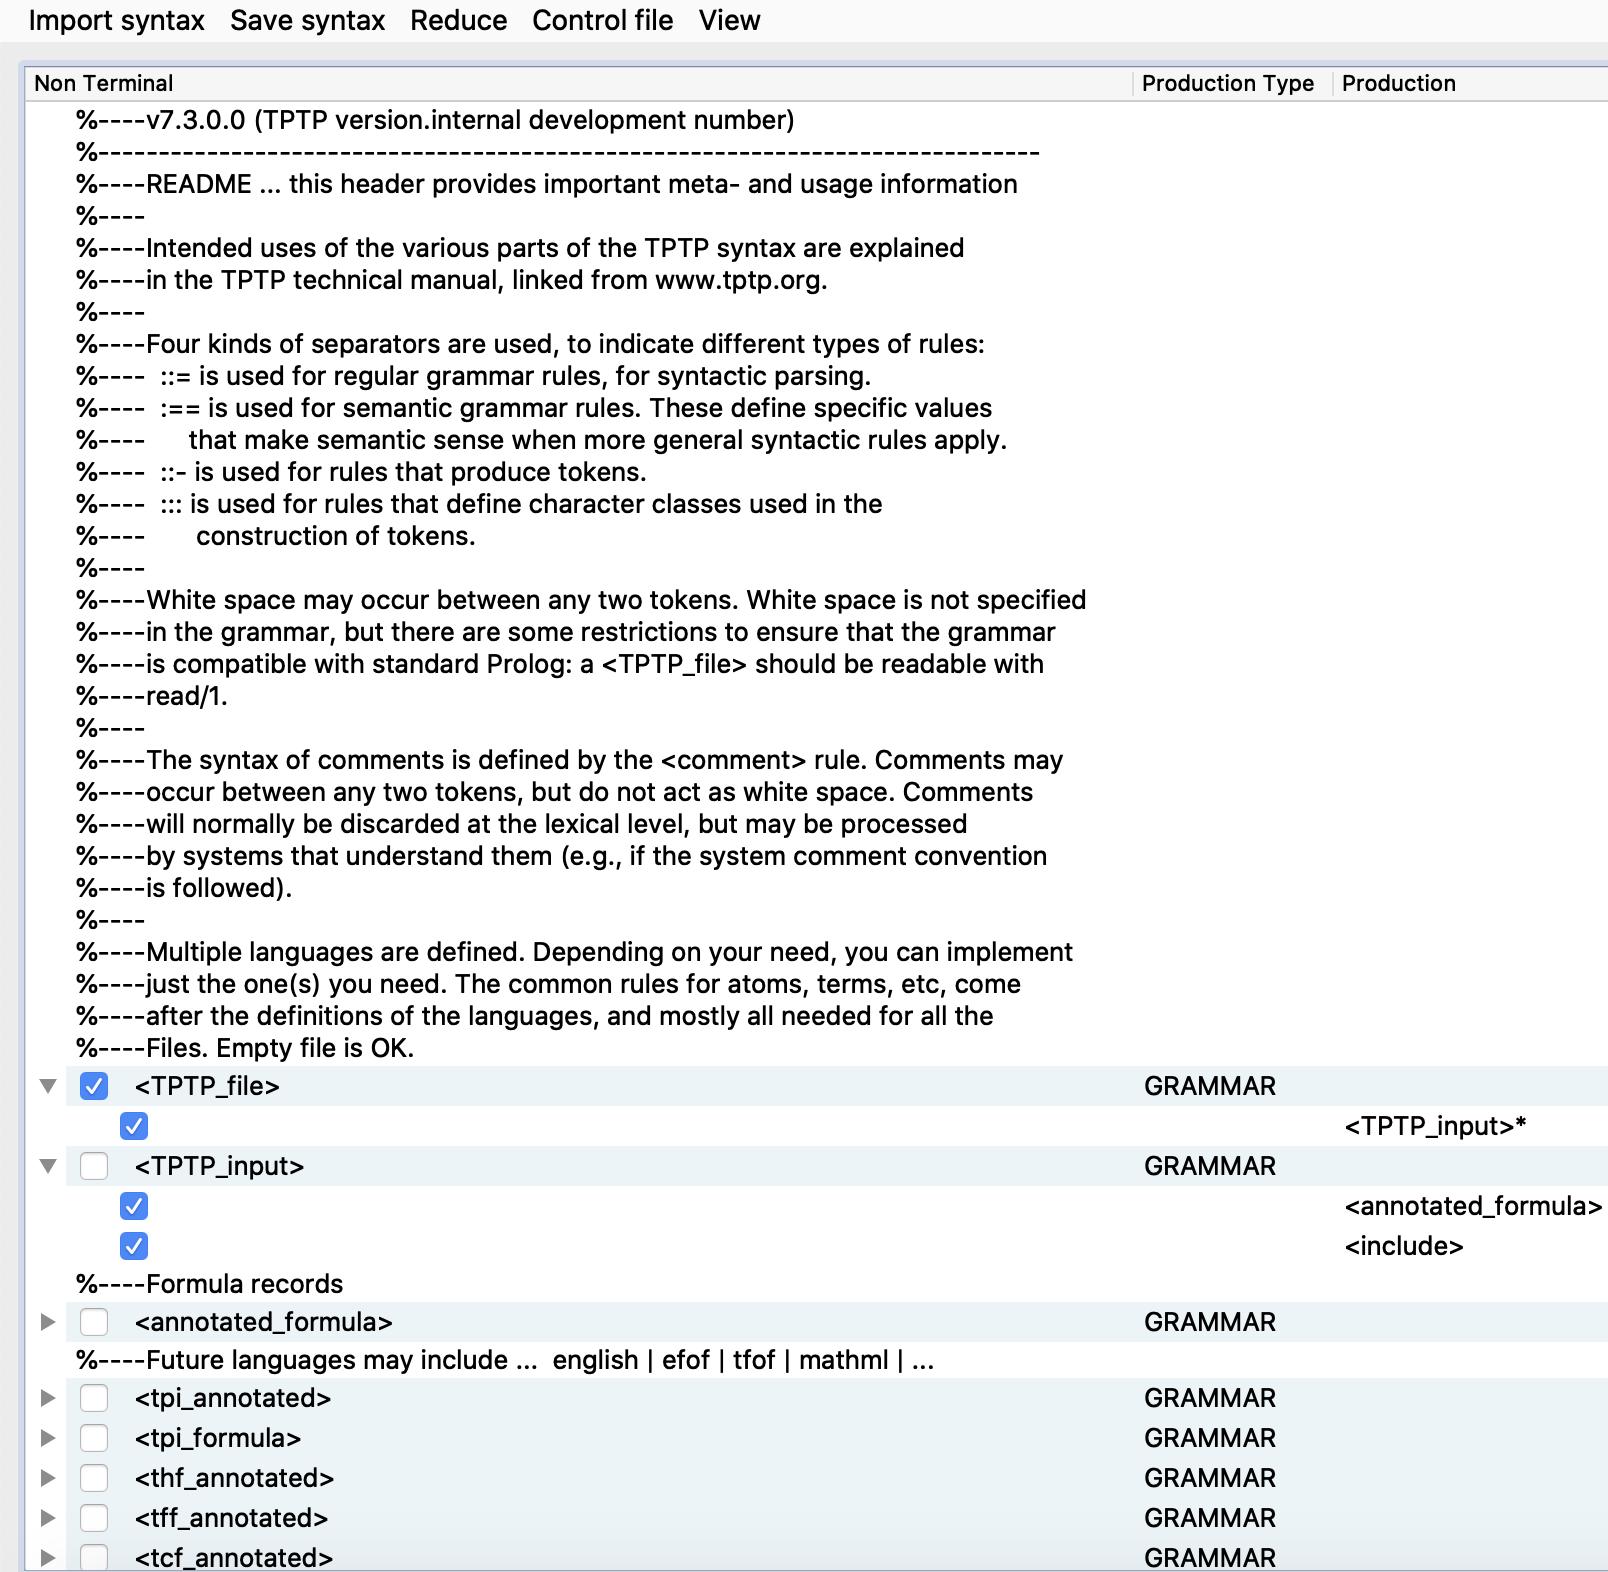
\includegraphics[width=1\textwidth]{images/gui.png}
\caption{GUI}
\label{fig:gui}
\end{figure}

The $View$ menu, shown in figure \ref{fig:view}, provides the possibility to toggle the display of comments to improve readability.

\begin{figure}[H]
\centering
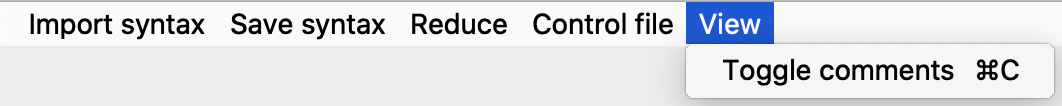
\includegraphics[width=.7\textwidth]{images/view.png}
\caption{View menu}
\label{fig:view}
\end{figure}

In order to extract a sub grammar the user has to choose a new start symbol by checking one of the check boxes left of the nonterminal symbols name. By default the start symbol that has been selected after importing the grammar is selected. For selecting blocked productions the user has the choice of on the one hand expanding the rules and uncheck the checkboxes belonging to the productions the user wishes to block. On the other hand the user can import a control file. If the user imports a control file the checkboxes are set accordingly.

In the $Reduce$ menu that can be seen in figure \ref{fig:reduce} the user can reduce the grammar according to his selections. The grammar is reduced and the reduced grammar is displayed afterwards. The rules maintain the same order as in the original TPTP grammar.

\begin{figure}[H]
\centering
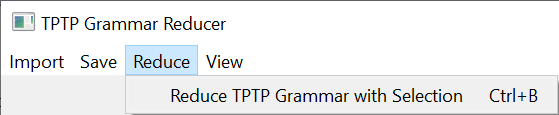
\includegraphics[width=.7\textwidth]{images/reduce.png}
\caption{Reduce menu}
\label{fig:reduce}
\end{figure}

In the $Save$ menu that is shown in figure \ref{fig:save} the user can reduce the grammar based on his GUI selection or an imported control file. The difference between the reduce option and the save menu is that the save menu saves the generated reduced grammar to local storage and does not display it. If the user wishes that the $\textless comments\textgreater$, which is necessary for using the automated parser generator, production is including in the reduced grammar the user has the option to save the reduced grammar with the $\textless comment\textgreater$ production.
The $Save$ menu also gives the user the option to generate a control file based on his GUI selection. This is particularly helpful if the users is reducing the same grammar multiple times. This way he can use the import control file option later instead of selecting the blocked productions in the GUI tool.

\begin{figure}[H]
\centering
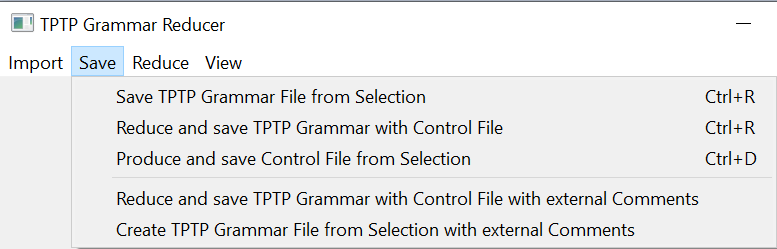
\includegraphics[width=.7\textwidth]{images/save.png}
\caption{Save menu}
\label{fig:save}
\end{figure}

todo
\begin{figure}[H]
\centering
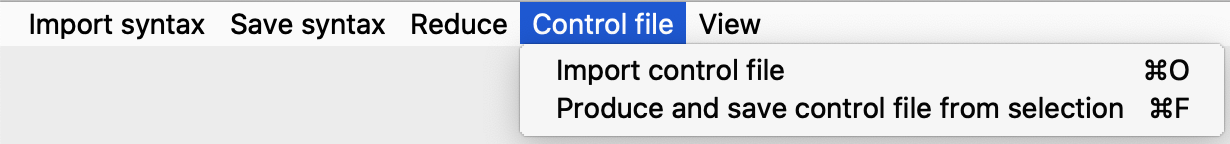
\includegraphics[width=.7\textwidth]{images/control_file_menu.png}
\caption{Control file menu}
\label{fig:ControlFileMenu}
\end{figure}

\section{Command-line interface}\label{sec:ConceptCommandLineInterface}
The goal of the command-line interface is to provide the means for convenient automation of sub-syntax extraction.
It takes a \ac{TPTP} syntax file and a control file as input and outputs the resulting sub-syntax.
Also basic help information is also accessible over the command-line interface.\\
Table \ref{tbl:ImplementationCommandLineParameters} provides an overview about the command-line arguments.
The syntax file location and the control file location has to be specified.
Specifying an output path and file name is optional, by default the output filename will be \textit{output.txt}.
The $-ex$ flag enables additional output of the comment syntax (see \ref{sec:ConceptAutomatedParserGenerator}.
Additionally, the help description can be opend by using the \textit{-h} option.
\begin{table}[H]
\centering
\caption{Command-line interface parameters}
\begin{adjustbox}{width=1\textwidth, center=\textwidth}
\renewcommand{\arraystretch}{2}
\begin{tabular}{llll}
\textbf{Name} & \textbf{Short form} & \textbf{Default} & \textbf{Description}\\\hline
-{}-grammar & -g & None & \ac{TPTP} syntax file path and filename\\
-{}-control & -c & None &  Control file path and filename\\
-{}-output & -o & output.txt & Output file path and filename (optional)\\
-{}-external\_comment & -ex & False & Flag to include external comment syntax (optional)
\end{tabular}
\end{adjustbox}
\label{tbl:ImplementationCommandLineParameters}
\end{table}

The implementation of the command-line interface is described in section \ref{sec:sec:ImplementationCommandLineInterface}

todo include comment option

 
-more complex actions like control file generation can more comfortably be done by using gui
-gui package not needed

todo count rules